\documentclass[../../main.tex]{subfiles}

%TODO: Da li obuhvatiti i registrovane korisnike da mogu uzivo? 

\begin{document}

\begin{longtable}{| p{.20\textwidth} | p{.80\textwidth} |} 
\hline
    Kratak opis &  Neregistrovani korisnik dolazi u teretanu da se prijavi na takmičenje. Recepcionar uzima njegove podatke i participaciju. \\ 
\hline    
    Učesnici & \begin{enumerate}
        \item Neregistrovani korisnik - Želi da se prijavi da učestvuje na takmičenju iako nije član teretane.
        \item Recepcionar - Želi da brzo izvrši prijavu novog takmičara.
    \end{enumerate}\\
\hline
   Preduslovi & \begin{enumerate}
       \item Sistem je u funkciji i recepcionar je ulogovan.
       \item Postoji aktivna prijava za takmičenje.
   \end{enumerate}\\
\hline  
    Postuslovi & \begin{enumerate}
        \item Korisnik je dobio broj prijave.
        \item Baza podataka je ažurirana.
    \end{enumerate}\\
\hline
    Osnovni tok & \begin{enumerate}
        \item Korisnik dolazi na recepciju i izjašnjava se da želi da se prijavi na takmičenje.
        \item Recepcionar ulazi u deo sistema vezan za takmičenja i bira opciju "Prijavi novog takmičara".
        \item Recepcionar traži potrebne podatke od korisnika i popunjava formular. 
        \item Nakon što popuni sva polja recepcionar pritiska dugme "Prijavi takmičara".
        \item Sistem proverava podatke i ispisuje cenu participacije i nudi izbor načina plaćanja.
        \item Recepcionar obaveštava korisnika o ceni participacije i pita za način plaćanja.
        \item Korisnik vrši plaćanje.
        \item Recepcionar potvrđuje plaćanje i zaključuje prijavu.
        \item Sistem obaveštava recepcionara da je prijava uneta u sistem.
        \item Recepcionar obaveštava korisnika da se uspešno prijavio. Daje mu račun i papir sa prijavom.
        \item Korisnik odlazi sa računom i prijavom.
    \end{enumerate}\\
\hline
    Alternativni tokovi & \begin{itemize}
        \item[A1] Pad sistema: Ukoliko u bilo kom trenutku dođe do pada sistema potrebno je obezbediti oporavak i čuvanje informacija. Recepcionar restartuje sistem i ponovo se uloguje. Slučaj se nastavlja na koraku 1.
        \item[A5] Neispravni podaci: Sistem obaveštava recepcionara koja polja su neispravna. Slučaj se nastavlja na koraku 3.
        \item[A6] Korisnik odustaje od prijave: Korisnik se izjašnjava da odustaje od prijave. Recepcionar pritiska dugme "Odustani". Korisnik odlazi iz teretane. Slučaj se ovde završava.
        \item[A7] Korisnik nema dovoljno sredstava za uplatu: Korisnik bira alternativni način plaćanja. Slučaj se nastavlja na koraku 7.
    \end{itemize}\\
\hline
    Podtokovi & Plaćanje participacije\begin{itemize}
        \item[7.1] Plaćanje gotovinom \begin{enumerate}
            \item Recepcionar bira opciju \textit{Plaćanje gotovinom}.
            \item Korisnik predaje recepcionaru novac.
            \item Recepcionar prebrojava novac i unosi sumu u sistem.
            \item Sistem ispisuje koliki je kusur.
            \item Recepcionar vraća kusur, ukoliko ga ima.
        \end{enumerate} 
        \item[7.2] Plaćanje karticom \begin{enumerate}
            \item Recepcionar bira opciju \textit{Plaćanje karticom}.
            \item Korisnik daje karticu recepcionaru.
            \item Recepcionar prislanja ili ubacuje karticu u aparat.
            \item Sistem upravlja plaćanjem i traži unos pin koda.
            \item Korisnik unosi pin kod.
            \item Sistem proverava informacije.
            \item Sistem beleži informacije o uplati.
            \item Recepcionar vraća karticu korisniku.	
        \end{enumerate}
    \end{itemize}\\
\hline
    Specijalni zahtevi & Teretana poseduje POS aparat za plaćanje karticom.\\
\hline
    Dodatne informacije & Informacije koje formular traži: ime, prezime, datum rođenja, e-mail, broj telefona i izbor disciplina.\\
\hline
\caption{Prijava na takmičenje uživo} % needs to go inside longtable environment    
\end{longtable}

\begin{figure}[!ht]
\begin{center}
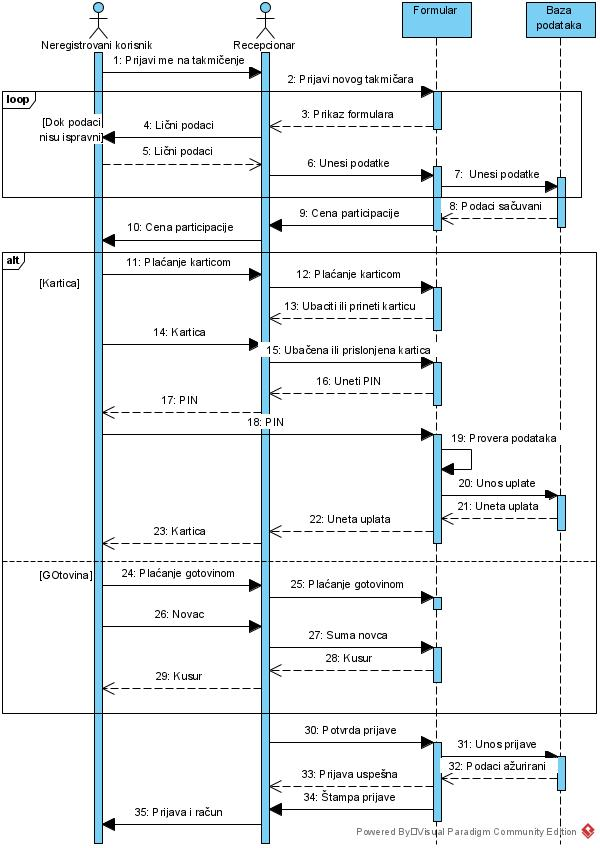
\includegraphics[scale=0.55]{sections/images/takmicenje_prijava_uzivo_dijagram_sekvenci.jpg}
\end{center}
\caption{Dijagram sekvenci za prijavu na takmičenje uživo}
\label{fig:kontekst}
\end{figure}

\end{document}
